\subsection{KOG Category Counts}
\label{sec:results.kogcount}

% Overview of KOG category distribution across the 114 plant proteomes

Due to the process of aligning each proteome against the 
reference model in KOG and the strict alignment criterion 
of 95\% minimum identity, many sequences of the Phytozome 
database don't find a matching pair in KOG. As expected, 
\emph{A. thaliana} is the best represented proteome from 
all 114 in the dataset, with a global coverage of 96.48\%, 
being the average and median coverage of 6.95\% and 
3.80\%, respectively. The next 
plants in the list are all Eudicots: \emph{A. halleri} (40.23\%), 
\emph{A. lyrata} (36.48\%), \emph{B. stricta} (22.79\%), and 
\emph{C. grandiflora} (21.69\%). The first Monocot and alga 
to appear are \emph{H. vulgare} (7.07\%) in the \nth{28} position 
and \emph{D. salina} (4.22\%) in the \nth{44} position, 
respectively. The least represented plants are 
\emph{A. trichopoda} (1.29\%), \emph{A. officinalis} (1.56\%), 
\emph{C. zofingiensis} (1.65\%), and \emph{D. carota} (1.69\%), 
each from a different biological category of the four 
defined in this study.

\begin{figure}[htp!]
\centering
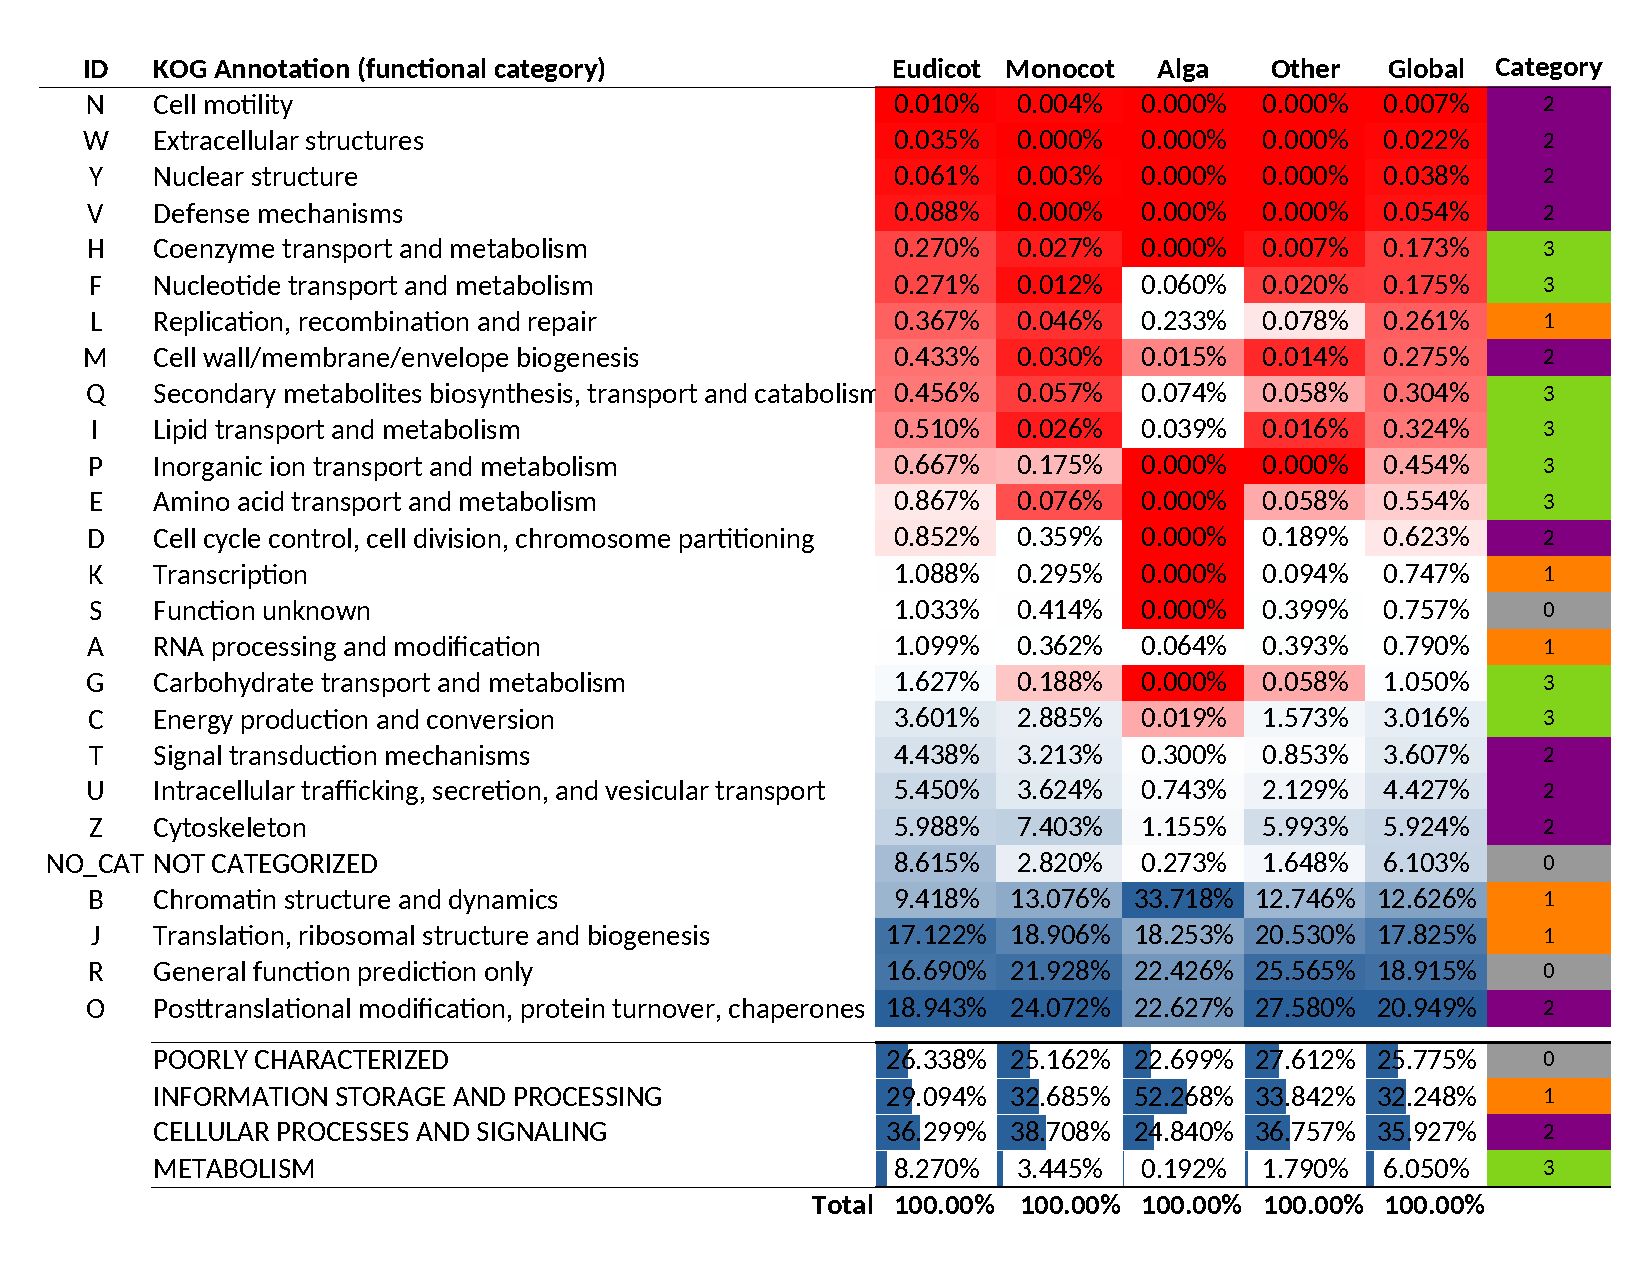
\includegraphics[width=\textwidth]{figures/Heatmap_EMAO}
\caption{Heatmap of the normalized KOG category frequencies 
observed in Phytozome, along with a summary of their 
functional relevance}
\label{fig:EMAO}
\end{figure}


Figure~\ref{fig:EMAO} shows the average of normalized frequency 
for the Phytozome Database. The KOG categories 
appearing the most are ``Posttranslational modification, 
protein turnover, chaperones" (O, 20.95\%), ``General function 
prediction only" (R, 18.91\%), ``Translation, ribosomal 
structure and biogenesis" (J, 17.82\%), and ``Chromatin 
structure and dynamics" (B, 12.62\%). The least frequent 
categories are ``Cell motility" (N, 0.007\%), ``Extracellular 
structures" (W, 0.022\%), and ``Nuclear structure" 
(Y, 0.038\%). The average and median normalized frequency 
for KOG categories are 3.84\% and 0.685\%, respectively. 

% Comparison of KOG category frequencies among different taxonomic groups (e.g., Monocots, Eudicots, Algae, etc.)
As seen in Figure~\ref{fig:EMAO}, the top 4 represented 
categories are still the same as the mentioned for the whole 
database, although the rank changes for Algae: now the most 
represented category is ``Chromatin structure and 
biogenesis". Especially for the Algae and Other groups, there 
is a lack of representation of several KOG categories, 
leading to red gaps in the shown heatmap.
Another interesting KOG category frequency to look at is 
``Carbohydrate transport and metabolism", because it 
allows distinction between Eudicots (1.63\%) and any other 
group (less than 0.2\%).

Note that the proportion of poorly characterized proteins 
is relatively high for the ``Other" group (around 25\%), 
which suggests a lack of established functional 
categorizations across this diverse cluster of species. 
Similarly, ``Information storage and processing" has a 
greater representation in Algae (52.3\%) than any other 
category. This variation implies potential differences 
in nuclear regulatory processes among these plants.

Another important insight is to look at translational 
and posttranslational processes (categories J and O, 
respectively). These two categories add up to more than 
36\% of in all biological groups, showing how significant the 
proteome acts toward these housekeeping tasks.


\subsection{Hierarchical Classification}
\label{sec:results.hierarchy}

% Presentation of the hierarchical organization of plant 
% species based on KOG counts

Before presenting the results of a hierarchical 
classification based on the KOG category counts, it is 
important to mention that the retrieved dataset consists 
mainly of Eudicotyledons (61.4\%) and Monocotyledons (25.4\%). 
The vast majority of Eudicots belong to the Rosids (56) 
and the Asterids clades (9). On the other hand, it can be 
observed on the taxonomic tree (Figure~\ref{fig:taxa}) 
that it encompasses a wide array of species 
spanning algae, mosses, ferns and flowering plants.

\begin{figure}[htp!]
\centering
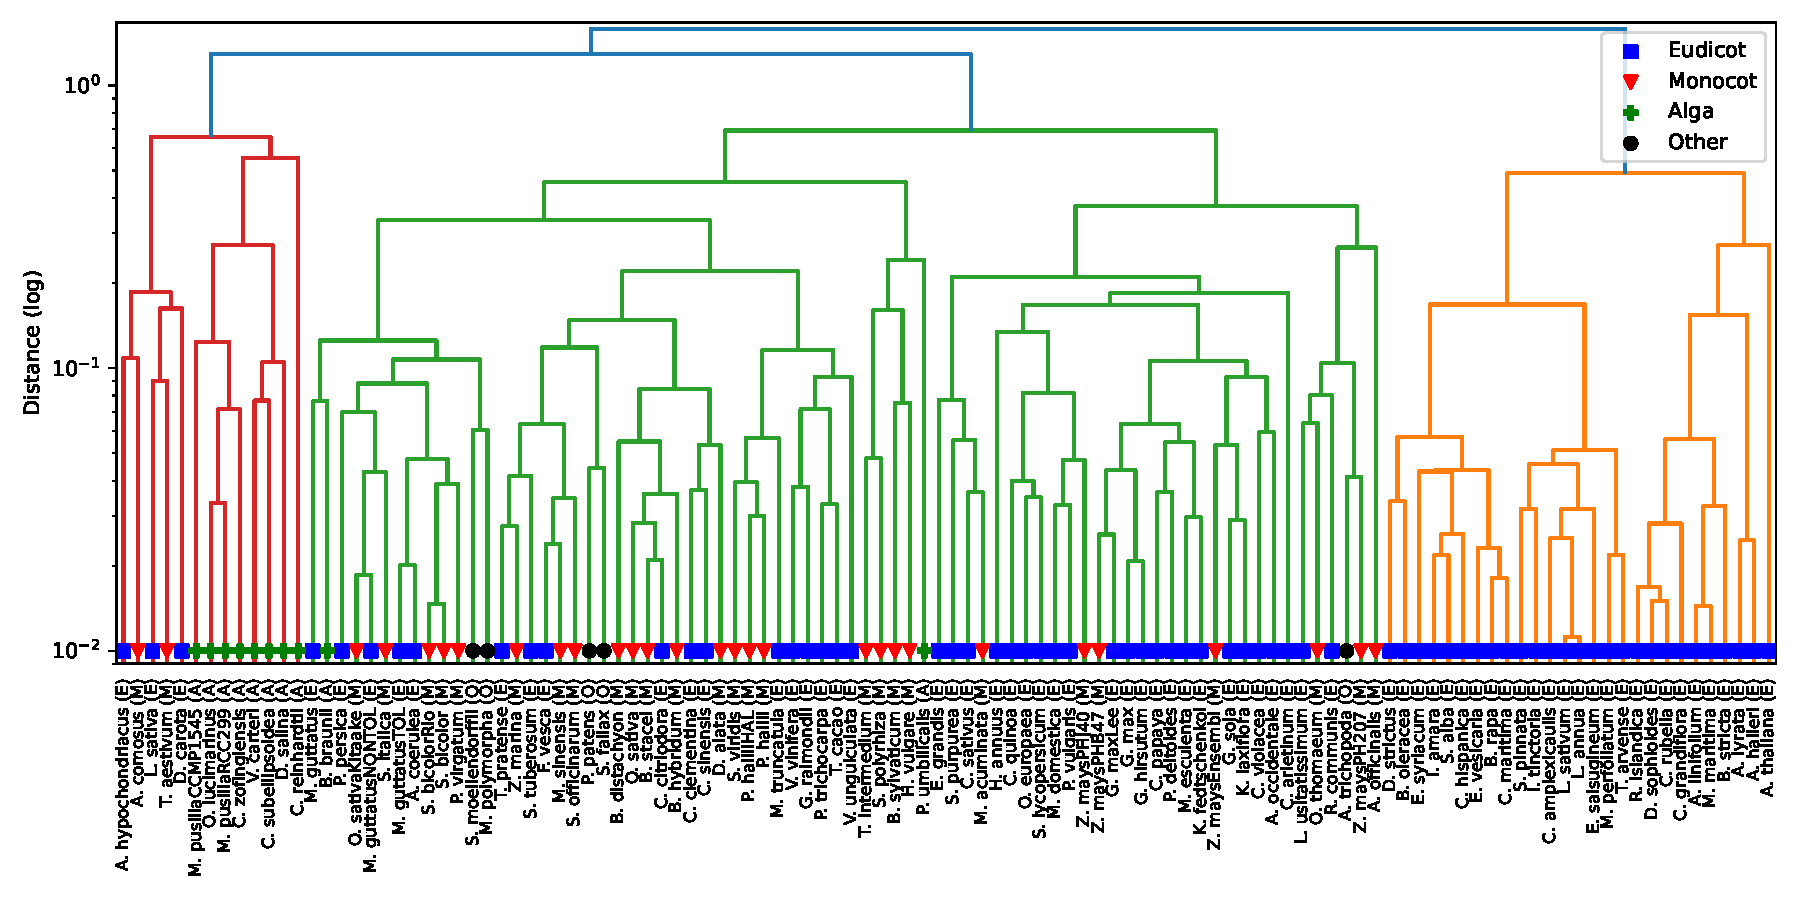
\includegraphics[width=1.1\textwidth]{figures/dendrogram_ward}
\caption{Dendrogram of the Phytozome proteomes, using KOG 
category frequencies as vector representations for 
computing euclidean distance}
\label{fig:dendrogram}
\end{figure}

% Discussion of the clustering patterns and their significance in elucidating plant evolutionary history
% Examination of species groupings and their agreement with known taxonomic classifications
Based on the obtained frequencies of KOG annotations (both 
relative and normalized), the corresponding hierarchical 
classification is carried out and the resulting 
dendrogram can be observed in Figure~\ref{fig:dendrogram}.
The first aspect that comes unnoticed are the red cluster at 
the left side including many algae and the 
Eudicots-only cluster shown in orange at the right side. 
While the former includes 5 non-algae and leaves out 
two algae, the latter is outstanding on the grounds 
that it perfectly groups all plants from the 
\emph{Brassicaceae} family, a part of the Rosids clade (See 
last 27 rows in Figure~\ref{fig:taxa}).

% Identification of interesting clusters and their potential evolutionary implications
Upon further analysis, it can be seen that the Other KOG 
category splits into \emph{A. Trichopoda}, and two groups 
of two plants each. Apart from those clusters, few relevant 
clusters of different or the same genera appear, beside from 
\emph{Arabidopsis}, \emph{Citrus}, and \emph{Sorghum}, which 
are correctly clustered.

Furthermore, Figure~\ref{fig:clustermap} displays a 
heatmap showing both a hierarchical clustering on the KOG 
categories as well as on the species, as previously depicted 
in detail. Further analysis of the clustering shows 4 clearly 
differentiated clusters, also related to the ranking shown in 
Figure~\ref{fig:EMAO}:

\begin{figure}[htp]
\centering
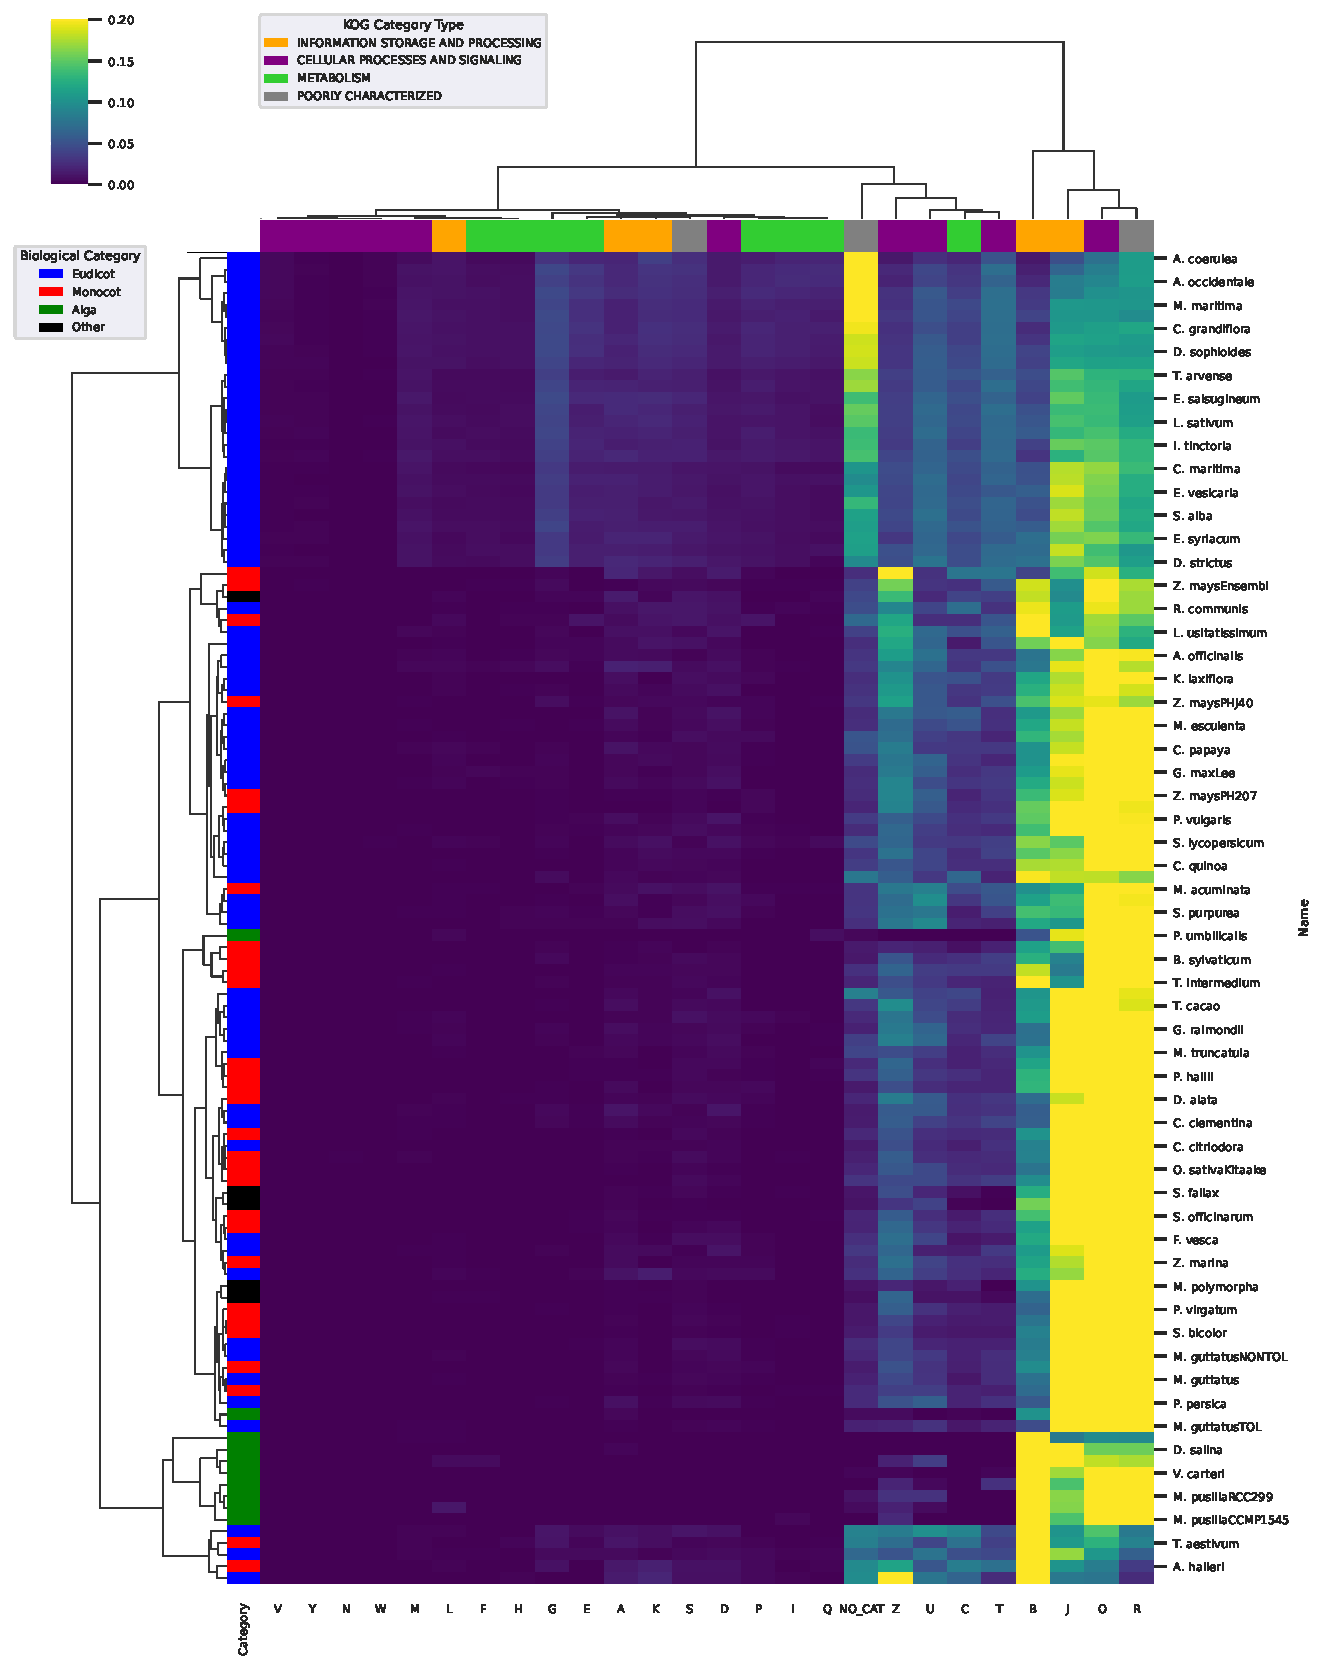
\includegraphics[width=\textwidth]{figures/clustermap}
\caption{Heatmap of the normalized KOG category frequencies 
observed in Phytozome, along with hierarchical clustering 
on categories and on species}
\label{fig:clustermap}
\end{figure}

\begin{enumerate}
\item Categories B, J, O, and R are the most abundant. A 
predominance of processes related to genetic information 
processing and regulation can be observed in this cluster.
\item Categories \verb|NO_CAT|, Z, U, C, and T follow the 
frequencies of previous cluster. This cluster revolves 
mostly around cellular dynamics and signaling, although the 
presence of \verb|NO_CAT| suggest a diverse set of functions.
\item Categories G, E, A, K, S, D, P, I, and Q suggest that 
this cluster is associated with diverse metabolic and 
regulatory processes, emphasizing cellular diversity and 
adaptability.
\item Categories V, Y, N, W, M, L, F, and H are related to 
cellular structure, integrity, defense and maintenance.
\end{enumerate}



\subsection{Comparison between Gene Ontology and Phytozome}
\label{sec:results.phytozome-go}

% Summary of the mean and standard deviation of KOG and GO category frequencies
After computing the relative and normalized KOG frequency 
counts for both Phytozome and GO proteomes, the analysis 
results are presented in Figure~\ref{fig:GO}. Note that 
although relative values are not very similar, 
the difference is almost indiscernible between the normalized 
frequency values for both databases. Furthermore, the result 
of using the Spearman's rank correlation coefficient is 0.98, 
suggesting minor differences between the two databases. The 
correlation coefficients shown below correspond to the 
computation against the normalized Phytozome ranking.

\begin{figure}[htp!]
\centering
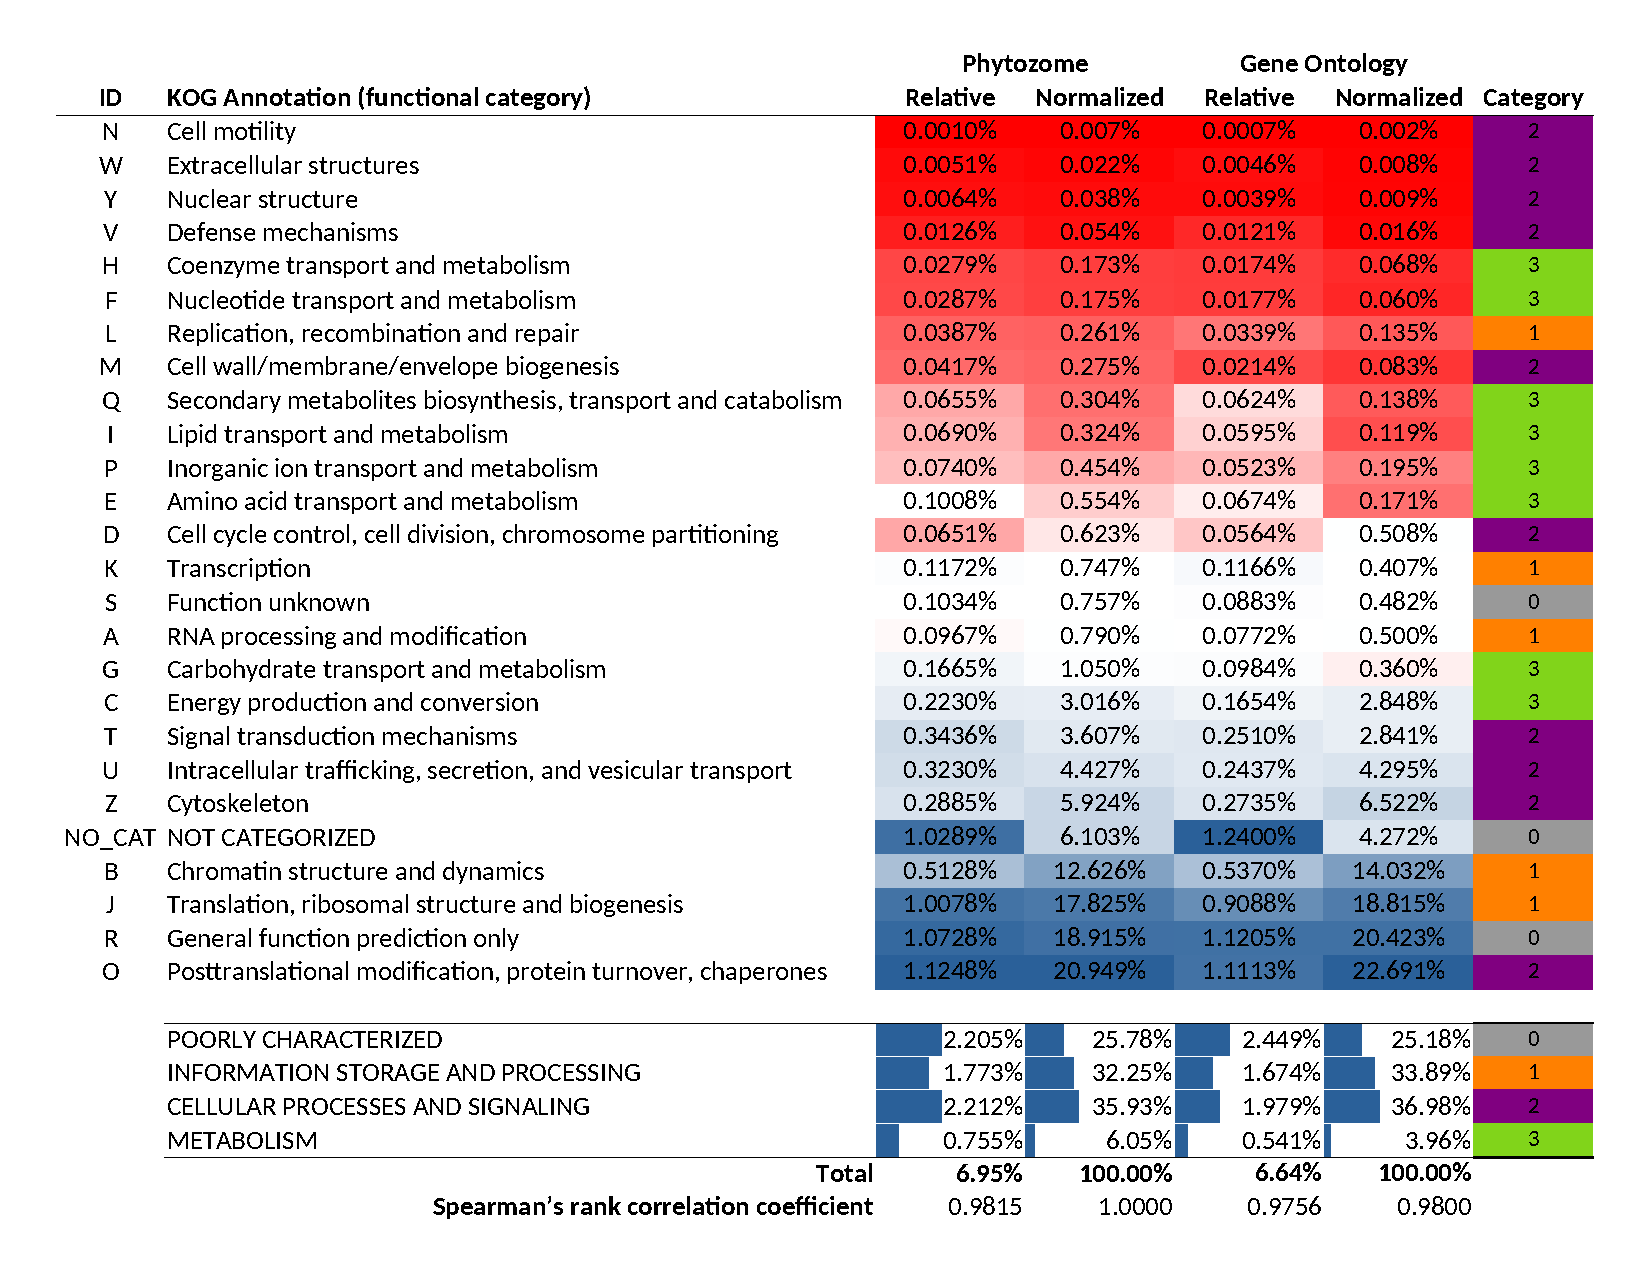
\includegraphics[width=\textwidth]{figures/Heatmap_GO}
\caption{Heatmap of the normalized KOG category frequencies 
observed in Phytozome and GO}
\label{fig:GO}
\end{figure}

Few categories change their relative order in the normalized 
GO ranking, such as ``Cytoskeleton (Z)", ``Carbohydrate 
transport and metabolism (G)", ``Cell cycle control, cell 
division, chromosome partitioning (D)", ``Inorganic ion 
transport and metabolism (P)", and 
``Cell wall/membrane/envelope biogenesis (M)". Besides, 
categories such as ``cell wall/membrane/envelope 
biogenesis (M)" and ``secondary metabolite biosynthesis, 
transport, and catabolism (Q)" show differential 
enrichment in Phytozome compared to Gene Ontology. 
This could indicate variations in the emphasis between 
the two databases.

